\section{Algorithm for near duplicate detection}
\label{section:luciv}

In the section the improved version of Luciv et.al. algorithm~\cite{luciv2019interactive} is presented.
The utilization of semi-local sequence alignment algorithms in algorithm phases improves overall time complexity.
%% We now describe an improved version of  by utilizing a \emph{semi-local sa} solution.
%% Then we present proof that improved version preserves completnesess property.
%% It is achieved by imitating all phases of the algorithm. 
It is also proved that the improved algorithm preserves all advantages of the initial one stated at~\cite{luciv2019interactive} such as search completeness.

\subsection{Algorithm description}

As the base one (see section~\ref{sec:lucivalgo} and~\ref{Luciv}), the presented algorithm consists of three sequential phases.
Moreover, each step of the presented algorithm imitates the corresponding step of the base one.
Aldorithm pseudocode is presented at Algorithm~\ref{alg:patternMathing1}.
% As the base one, the presented algorithm comprises three phases.

At the first phase (lines 1-3) semi-local sa problem is solved for pattern $p$ against the whole text $t$.
This solution provides access to the string-substring matrix $H^{str-sub}_{p,t}$ which allows performing fast queries of \emph{sa} score for pattern $p$ against every substring of text $t$.
Then, we construct matrix $M$ by applying transposition and inverse operation implisitly on $H^{str-sub}_{p,t}$:
$$M[j,i]:= -H^{str-sub}_{p,t}[i,j].$$
Note, transposition operation preserves (anti) Monge property whereas inverse operation transforms anti-Monge matrix into the Monge one and vice versa. 
Thus, $M$ is a Monge matrix.

The second phase comprises several steps (lines 4--6).
First, we want to get for each prefix of the text $t$ the longest suffix that has the highest similarity with the given pattern $p$ with the following constraint.
The lengths of obtained suffixes should be in $[|p|*k..\frac{|p|}{k}]$ interval where $k \in (\frac{1}{\sqrt{3}},1]$.
It could be done in several ways.
For example, direct pass through diagonal with width $w:= \frac{|p|}{k} - |p|*k = |p|(\frac{1}{k} - k)$ in $H^{str-sub}_{p,t}$ or in $M$ (Fig. \ref{fig:M2}).
Another approach is the following.
Note, $M$ is a Monge matrix where indices are swapped with respect to matrix $H^{str-sub}$.
Thus, diagonal can be covered, with 1 step discreteness, by approximately $ | t | $ square windows of size $ w \times w $.
Because of length constraint, we are only interested in elements that lie in the main diagonal and below it (remember, transposition) in these submatrices $w\times w$.
Each of these submatrices is Monge by definition, as a submatrix of a Monge matrix.
Hence, $W$ is totally monotone.
Moreover, determining all elements lying above the main diagonal to be $+\inf$ preserves total monotonicity.
Thus, the \textrm{SMAWK} algorithm\cite{.} can be applied to this matrix in order to find a leftmost element that has a minimum in a given row with the corresponding column position.
In our case, leftmost means that for each prefix algorithm detects the longest suffix.

%\begin{figure}[H]
%	\centering
%   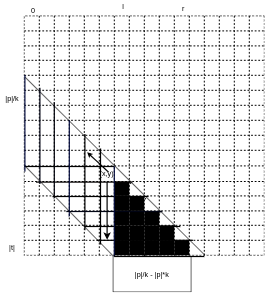
\includegraphics[width=0.4\columnwidth]{figures/M2.png}
%    \caption{Диаграмма компонентов системы}\label{fig:M2}
%\end{figure}

The second step, it is one-way pass through these suffixes with a sliding window of size $\frac{|p|}{t}$ to find for each window that has alignment score greater or equal to given threshold $-k_{di}$ with pattern $p$ most similar suffix with the longest length. 

The third phase (lines 7--11) is the same as in the base algorithm.

\begin{algorithm}[!t]
\caption{PATTERN BASED NEAR DUPLICATE
SEARCH ALGORITHM VIA SEMI-LOCAL SA}
\label{alg:patternMathing1}
Input: pattern $p$, text $t$, similiarity measure $k \in  [ \frac{1}{\sqrt{3}} ,1  ]$\\
Output: Set of non-intersected clones of pattern $p$ in text $t$
\begin{equation}
    k_{di}=|p|*(\frac{1}{k}+1)(1-k^2)
\end{equation}
\begin{equation}
 L_{w} = \frac{|p|} {k}
\end{equation}
\begin{equation}
  w = |p|(\frac{1}{k} - k)
\end{equation}
Pseudocode:
\begin{algorithmic}[1]
\STATE{$W = semilocalsa(p,t)$}
\COMMENT{1st phase}
\STATE{$H^{str-sub}_{p,t} = semilocalsa(p,t).stringSubstringMatrix$}
\STATE{$M[j,i] = -H^{str-sub}_{p,t}[i,j]  $}
\STATE{$sufixes = processDiagonal(M,L)$}
\COMMENT{2d phase}
\STATE{$W_2 = SuffixMaxForEachWindow(sufixes,L_{w})$}
%% \STATE{$filter(W_2,k_{di})$}
\STATE{ $W_3 = UNIQUE(W_2)$}
\COMMENT{3rd phase unchanged}
\FOR{$w \in W_3$}
\IF{$\exists w^{'} \in W_3:w \subset w^{'} $}
\STATE{ $remove$ $w$ $from$ $W_3$}
\ENDIF
\ENDFOR
\RETURN $W_3$
\end{algorithmic}
\end{algorithm}

\begin{theorem}
Algorithm \ref{alg:patternMathing1} runs in $max(O(|t|*|p|),\ O(|t| * \log |t|))$ time with $O( |t| \log |t|)$ additional space where $p$ is pattern, $t$ is text, $|p| \leq |t|$, and $v=O(1)$ where $v$ is denominator of normalized mismatch score for semi-local sa $w_{normalized} = (1,\frac{\mu}{v},0)$.
\end{theorem}
\begin{proof}
  For each phases of algorithm we provide it's time and space bounds.
  
\emph{First phase.}
We store solution $H$ of \emph{semi-local sa} by decomposing it to permutation matrix $P$ of size $O(v*|t| \times v*|t|)$ (lines 1-3, Theorem~\ref{decomposition}).
The permutation matrix can be stored via two permutations of size $v*|t|$ for columns and rows.
It is simply two lists of size $v*|t|$.
Then, for random access query in specific position $(i,j)$ of matrix $H$ one need to check how many points are dominated by $H [i,j]$.
It can be done by checking all points of permutation matrix and requires $O(v * |t|)$ steps.
Thus, the total time and space complexity of the first phase are $O(v *|p| * |t|)$ (time needed to solve semi-local sa) and $O(v*|t|)$ respectively.
Given $v=O(1)$ we have $O(|p| * |t|)$ and $O(|t|)$ respectively.
% Also, note, in our case, random access query runs in time $O(|t|)$.
% kernel $P$ has at most $v*|t|$ non zeros (after we use $blow-up$ technique for transition  to \emph{semi-local lcs}).
%Due to the fact that $v = O(1)$, $O(v*|t|)$ becomes $O(|t|)$.
%Note that for such simple data structure we need to calculate the number of %points that dominated by given point to make random access to $P$. It requires %checking at most   $O(|t|)$ points. 

%The solution of \emph{semi-local sa} when $v=O(1)$ is just $O(|t|*p)$.

%The total bounds for time and space complexity for this phase are at most $O(|t|*|p|)$ and $O(|t|)$ correspondingly.

\emph{Second phase}.
For the sake of clarity, we omit $k$ factor in algorithm analysis since $k$ is just a constants within interval $(\frac{1}{\sqrt{3}},1]$.
In the proof, we follow the first approach described in the algorithm description for this phase.
First, we need to access the cell that represents substring $t_{0,|p|*k}$.
Note, such a random access query to a matrix element requires $O(|t|)$ time.
Further, by  proposition~\ref{incremental} we access adjacent elements for given cell $M[i,j]$ by $O(1)$.
Thus, we can traverse through the diagonal of matrix $M$ in time $O(|t|*|p|)$ iteratively as follows.
Let $(i',j')$ denotes the current position.
We process the $i'$-th row starting from position $j'$ until maximum length is reached, i.e. until $i^{'}-j \geq |p|*k$.
% Process row $i^{'}$ with starting $j^{'}$ (recall it cell by $M[i^{'},j^{'}]$) position  (go right i.e increment $j^{'}$) until $i^{'}-j \geq |p|*k$.
When the row is processed we shift by one $i^{'}$ down and $j^{'}$ to right of $(i',j')$ for the next iteration if needed (see \todo{picture} \red{This about the top left corner}).
% Then shift by one $i^{'}$ down and $j^{'}$ to right by one if needed (see picture \red{This about the top left corner}).

Each raw is processed twice.
First, to detect a maximum score.
Second, to find the longest suffix with the highest similarity.
%% When we pass through a slice of the specific row in diagonal $M$,  we also will find the longest suffix with the highest similarity simply by checking elements twice.
%% First for detect maximum score, second for detect the longest suffix among those who have this score.
%It requires storing at most $O(p)$ cells for each column but we only process one column at the time, thus, we will require only $O(p)$ additional space for that whole cell processing.
Thus, for storing for each prefix its longest suffix we need additionally $O(|t|)$ space.
Let $l^{prefs}$ denotes a list of stored prefixes.
Additionally, for each substring of length $\frac{p}{k}$ we store similarity score by querying them during diagonal passage.
Let's denote it by $C$.
Thus, at the end of the diagonal processing (line 4) $O(t)$ suffixes are collected and they require $O(t)$ space for storing.
Hence, the overall diagonal processing (line 4) requires $O(|t|+|t|*|p|) = O(|t|*|p|)$ time with $O(|t|+|p|) = O(|t|)$ additional space.

Further (Line 5), we again traverse each element of list $l^{prefs}$ with one step sliding window of size $L_w$.
For each windows we check wheather it satisfies the similarity criteria, i.e. its similarity score is at most $-k_{di}$.
The check can be performed by a simple lookup for a specific element of $C$ at $O(1)$.
If so then then we need $O(|p|)$ lookups within suffixes to query the most similar and longest one.
%% Further (Line 5), we need to find the longest suffix for each $O(|p|)$ windows with step one in applied to list of size $|t|$ with additional condition that within each window of size $O(\frac{|p|}{k}-|p|*k)=O(|p|)$ the suffix with length $L_{w}$ have similarity score at least $-k_{di}$.
%% It is simply a one-way pass-through list of suffixes where the processing of each window requires at most $O(|p|+1)=O(|p|)$.
%% More precisely, first, we check that for current window of size $O(|p|)$ its associated suffix has similarity not less then given threshold $k_{di}$.
%% It is simply lookup for a specific element in $C$ with $O(1)$.
%% If that true, then we need $O(|p|)$ lookups within $suffixes$ to query the most similar and longest one.
The total number of such windows can be approximated as $O(|t|)$.
Thus, the step (line 5) requires $O(|t|)*O(|p|) = O(|t|*|p|)$ computation time with $O(|t|)$ space.
%% The filtering process (Line 6) is a one-way pass through a list of suffixes $W_2$.
%% It requires at most $O(t)$ time.

Thus, the total running time and space complexity of the second phase is $O(|t|*|p|)$ and $O(|t|)$ respectively.

\emph{Third phase}.
The third phase remains unchanged, thus have the same time and space bounds as in the base algorithm case.
Note, it possible to perform this phase in-place during the second phase which speedups the algorithm, i.e decreases space and time complexity to $O(|t|)$ and $O(|t|*|p|)$ respectively.
The third phase can be approximated as $O(|t| * log|t|)$ for both space and running time complexity.

Thus, the total alforithm running time is $max(O(t * p),\ O(t * \log t))$ while space complexity is $O(t * \log t)$.
%% \red{It be good if we also improve third phase)))}
\end{proof}

\begin{theorem}
Algorithm \ref{alg:patternMathing1} with scoring scheme $w = (0,-2,-1)$ preserves completnesses property of algorithm~\cite{luciv2019interactive} and has running time and space complexity $max(O(t*p),\ O(t* \log t))$ and $O(t *  \log t)$  respectively.
\end{theorem}

\begin{proof}
Edit distance in the base algorithm~\cite{.} may be expressed as sequence alignment with following scoring scheme: 
$$w_{sa}=(w_{+},w_{0},w_{-}) = (0,-2,-1).$$

First, to get intial edit score we need to apply inverse operation:
$$editscore(a,b) = -sa(a,b,w_{sa}).$$
Next, $w_{sa}$ may be normalized using normalization~\ref{weightNormalization}:
$$(0, -2, -1) \rightarrow (1,\frac{\mu=0}{v=1}, 0).$$
\todo{equivalent? Thus, $d_{di} \leq k_{di}$ is the same as $sa \geq -k_{di}$.}

Second, let's carefull review phases 1 and 2 of given algorithms.
The base algorithm passes through the text with a sliding window to detect those fragments of size $L_{w}$ which have edit score above given threshold $k_{di}$.
Then within these fragments algorithm detects longest suffixes that are most similar to pattern $p$ with size within interval \todo{$I=pk...L_{w}$}.
The presented improved algorithm proceeds in a very similar way but, informally, phases are swapped.
First, it detects the longest suffixes with size in interval $I$ for each prefix of the text.
Then, it proceeds in such way that for each window of size $L_{w}$ that has alignment score with pattern $p$ below given threshold $-k_{di}$  the longest suffix most similar to $p$ is detected.
Due to \todo{formula~\ref{editsa}} results of the second phases of the algorithms are equal.
The third phase remains unchaned in the presented algorithm.
%% Thus, the presented algorithm preserves completeness.
Thus, the presented algorithm is complete.
For $w = (0,-2,-1)$, $v=1$ and algorithm running time and space complexity are as claimed.
%% For given $w = (0,-2,-1)$ we have $v=1$ then wehave running time as claimed.
\end{proof}

%At first algorithm \ref{luciv} pass through text $t$ with sliding window to detect those fragments which has similarity abobe given threhsold $k_{di}$ with size $\frac{p}{k}$.
%Then within these fragments algorithm detects longest suffixes most similar to pattern $p$ with size within  $pk...\frac{p}{k}$ interval.
%That how $A_1$ constucted.
%
%T%he second algorithm \ref{alg:patternMathing1} proceed in similar way but it first .
 .
%$Then filtering is perfomed in that way that only$
%That how $A_1$ constucted.
%those lonh suffices  left 
 %for those windows of size $\frac{p}{k}$ the longest suffix is left.

%T%%hus, $A_1=A_2$  by resulting equivalence of construction. 

